\documentclass{article}
\usepackage[T2A]{fontenc}    
\usepackage[russian]{babel}
\usepackage{multicol}
\usepackage{amsmath}
\usepackage[a4paper, total={5in, 8.5in}]{geometry}
\usepackage{makecell}
\usepackage {graphicx}
\usepackage[rightcaption]{sidecap}
\usepackage{wrapfig}
\usepackage[export]{adjustbox}
\usepackage{titling}
\usepackage{lipsum}
\usepackage{fancyhdr}

\makeatletter
\def\@maketitle{%
    \newpage
    \null
    \vskip 12em
    \vspace*{\droptitle}
    \maketitlehooka
    {\@bspreauthor \@author \@bspostauthor}
    \maketitlehookc
    \vspace{2mm}
    {\@bspretitle \@title \@bsposttitle}
    \maketitlehookd
    \par}
\makeatother

\pretitle{\par\noindent\bfseries\LARGE}
\posttitle{\par\vskip1em}
\preauthor{\par\noindent\large}
\postauthor{\hfill}
\predate{\Large}
\postdate{\par\vskip0.8cm}
 
\author{\footnotesizeЗ.Литовченко}
\title{Лучший вариант}
\graphicspath {  { ./images/ }  }
\date{}
\textwidth=15cm
\pagestyle{fancy}
\fancyhf{}
\rhead{\thepage}
\begin{document}
\setcounter{page}{12}
\begin{center}
Федеральное государственное автономное образовательное учреждение высшего  \\
образования \\
«Санкт-Петербургский национальный исследовательский \\
университет информационных технологий, механики и    оптики»\\
\vspace{1cm}
Кафедра Вычислительной Техники \\
Дисциплина: Информатика \\ \vspace{5cm}
Лабораторная работа №6 \\
Работа с системой компьютерной вёрстки \TeX \vspace{5cm}
\end{center}
\begin{flushright}
Баянов Равиль Динарович \\
Р3134 \\
\end{flushright}
\null\vfill
\begin{center}
Санкт-Петербург \\ 
2022
\end{center}
\newpage
\hrule
\begin{multicols}{2}
\maketitle

\noindent
Представьте себе, что вы --- директор школы-интерната, и вам нужно составить меню для столовой на неделю. Детальное составление меню, конечно, дело повара но вот проследить за тем, что денег будет истрачено не слишком много,нужно вам. \par
Вам известно, какие продукты можно купить, и их цены. Но, кроме цен, у них есть ещё множество качеств, например, калорийность, содержание тех или иных витаминов и т. п. Поэтому, кроме цен, при покупке продуктов вам нужно учитывать довольно много условий. Если к тому же на складе много продуктов, то задача становится весьма запутаной и без вычислительной машины решить её трудно. Однако, Если продуктов и условий мало, справиться с ней несложно. \par
Рассмотрим такой пример. Пусть меню уже почти полностью составлено, и вам нужно проследить только за тем, чтобы в нём оказалось достаточно витаминов A и C, причём на складе есть вишни и абрикосы. Один \par
\hspace{51mm} Таблица 1
\begin{flushleft}
\begin{tabular}{ | l | c | c |}
    \hline\rule{0mm}{5mm}
    \diaghead{\theadfont{Витаминиоррллоы}}
    {Фрукты}{Витамины} &
    \thead{A (г в 1 кг)}&\thead{C (г в 1 кг)}
    \\[5mm]\hline\rule{0mm}{6mm}
    \thead{Вишни} & \thead{3} & \thead{150}
    \\[5mm]\hline\rule{0mm}{6mm}
    \thead{Абрикосы} & \thead{24} & \thead{75}
    \\[5mm]\hline
\end{tabular}
\end{flushleft}
\vspace{10mm}
килограмм вишен стоит 25 коп., один килограмм абрикосов --- 30 коп., а содержание витаминов приведено в таблице 1. Вам нужно, чтобы недельный рацион содержал не меньше 6 кг витамина A и не меньше 75 кг витаминов на C. Сколько нужно купить вишен и абрикосов, чтобы выполнялись эти условия и затраты были минимальны? \par
Прежде всего задачу нужно сформулировать математически. Итак, пусть в рацион войдут x кг вишен и y кг абрикосов. Их стоимость составит $0,25 x+0,3 y$ рублей, содержание витамина A --- $0,003 x+0,024 y$ кг, а витамина C --- $0,15 x+0,075 y$ кг. Нам нужно найти такие x и y, для которых выполняется система неравенств
\begin{equation}
    \begin{cases}
        0,003x+0,024y\geq6,
        \\
        0,15x+0,075y\geq75,
        \\
        x>=0, y\geq0,
    \end{cases}
\end{equation}
и $z=0,25 x+0,3 y$ было бы минимальным. На плоскости xOy легко указать множество точек M, удовлетворяющих системе (рис. 1). Его называют \textit{многоугольником решений} системы. Ясно, что прямые $z=0,25 x+0,3 y$ при различных z параллельны одному и тому же направлению, причём при росте z они удаляются от начала координат. Поэтому нам нужно найти ту из прямых этого направления, которая имеет с многоугольником M общую точку и ближе всего к началу координат. Легко сообразить, что такая прямая не до лжна пересекать M по внутренним точкам --- тогда бы она не была самой <<низкой>> (рис. 2). Следовательно, она должна проходить через одну из вершин многоугольника. Но тогда эта точка - вершина C. Итак, нужно купить 400 кг вишен и 200 кг абрикосов --- лучший вариант найден!\\
\par

\begin{scriptsize}
    Задачи, подобные разобранной, называются \textit{задачами линейного программирования}. В них требуется найти прямую (в трёхмерном пространстве ----- плоскость, в многомерном - так называемую гиперплоскость), принадлежащую пучку параллельных прямых (плоскостей, гиперплоскостей), которая пересекается с некоторым многоцугольником (многогранником) и находится ближе всего (или дальше всего) от начала координат. Можно дать и чисто алгебраическую фор 
\end{scriptsize}
\end{multicols}
\begin{center}
    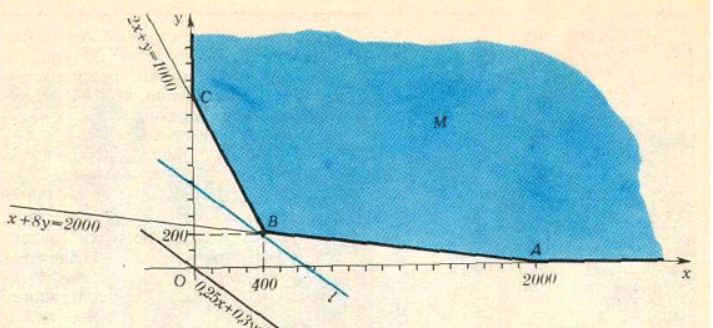
\includegraphics[width=1\textwidth]{./images/graphic1.png}
    \caption{рис. 1}
\end{center}
\begin{multicols}{2}
\begin{flushleft}
    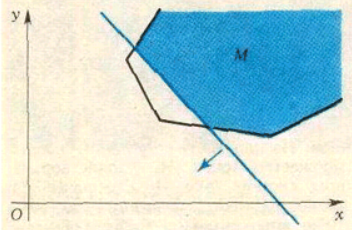
\includegraphics[scale=0.8]{./images/graphic2.png}
\end{flushleft}
\begin{scriptsize}
    мулировку: имеется система линейных неравенств
    
    \begin{math}
        \begin{cases}
            a_{11}x_1+a{12}x_2+\cdots+a_{1n}x_n\geq b_1,
            \\
            a_{21}x_1+a_{22}x_2+\cdots+a_{2n}x_n \geq b_2,
            \\
            . . . . . . . . . . . . . . . . . . . . . . . . . . . . . . . . . . . . . . . . . . . . . . . . . . 
            \\
            a_{k1}x_1+a_{k2}x_2+\cdots+a_{kn}x_n \geq b_k
        \end{cases}
    \end{math}
    
    \noindent
    и \textit{линейная} функция $z=c_1x_1+...+c_nx_n$. Нужно найти такое решение этой системы, для которого значение функции z минимально. О линейном программировании в <<Кванте>> было уже много сттей (1971 --- №3, с. 1 и №4, с. 1, 1974 --- №7, с.13, 1975 --- №10, с. 17, 1976 --- №7. с. 2, 1977 --- №8, с. 29).
\end{scriptsize}
нужно вырастить песцов и лисиц, чтобы средняя стоимость одной шкурки была минимальна, если стоимость выращивания одной лисицы --- 45 руб., а одного песца --- 25 руб.? \par
Решение. Пусть  x --- число выращиваемых лисиц, а y --- песцов. Тогда
\begin{equation}
    \begin{cases}
        4x+5y\leq80000
        \\
        \frac{1}{2}x+y\leq10000
        \\
        x\leq3000
        \\
        y\leq6000.
    \end{cases}
\end{equation}
Средняя стоимость одной шкурки
\[z=\frac{45x+25y}{x+y}.\]
Как вы видите, здесь функция, значение которой нам нужно сделать минимальным, не является линейной. Она задаётся отношнием двух линейных функций. Таки функции называются \textit{дробно-линейными}.
\end{multicols}
\fancyfoot{}
%\fancyfoot[LE,RO]{\thepage}
\pagestyle{empty}
\setcounter{page}{13}
\end{document}
